\documentclass[twocolumn]{article}
\usepackage{pgfplots, pgfplotstable}
\pgfplotsset{compat=newest}
\usepackage{amsmath}

\begin{document}

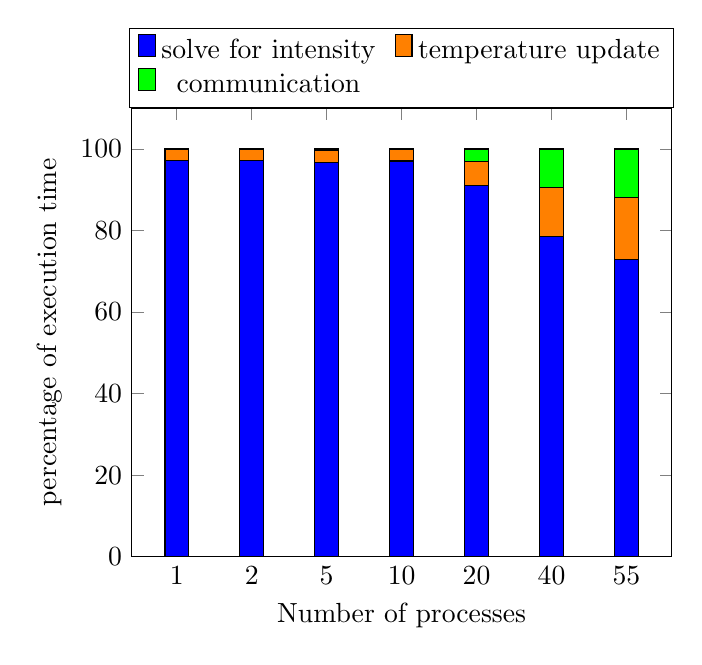
\begin{tikzpicture}
  \begin{axis}[
    ybar stacked, ymin=0,  
    bar width=3mm,
    symbolic x coords={1,2,5,10,20,40,55},
    xtick=data,
    xlabel=Number of processes,
    ylabel=percentage of execution time,
    legend columns=2,
    legend style={  at={(0.5,1)},
        /tikz/column 2/.style={
            column sep=5pt},
        anchor=south}, 
    ]
  ]

%97.25842754	2.741536712	3.57436E-05
%97.14934819	2.848848741	0.001803069
%96.70857988	3.069526627	0.221893491
%97.07485407	2.831618667	0.093527268
%91.13192131	5.832442964	3.035635724
%78.48410758	12.14343928	9.372453138
%72.83987024	15.33470953	11.82542023

  \addplot [fill=blue] coordinates {
({1},97.25842754)
({2},97.14934819)
({5},96.70857988)
({10},97.07485407)
({20},91.13192131)
({40},78.48410758)
({55},72.83987024)};
\addlegendentry{solve for intensity}
  \addplot [fill=orange] coordinates {
({1},2.741536712)
({2},2.848848741)
({5},3.069526627)
({10},2.831618667)
({20},5.832442964	)
({40},12.14343928)
({55},15.33470953)};
\addlegendentry{temperature update}
  \addplot [fill=green] coordinates {
({1},0.000035743)
({2},0.001803069)
({5},0.221893491)
({10},0.093527268)
({20},3.035635724)
({40},9.372453138)
({55},11.82542023)};
\addlegendentry{communication}
  
\end{axis}
\end{tikzpicture}

\end{document}